% Provenance (never printed): cycle 4 SVT, "La planete Terre, l'environnement
% et l'action humaine": resources from the Earth, their geological origin, the
% time they take to form and the rate we use them; see
% sources/book1/PROVENANCE.md. Book 1, grade 9, chapter 3.
% Vocabulary guard: owns ore deposit (with concentration factor), aggregate,
% reserve. Resource, renewable resource, ore, raw material (chemistry grade
% 5), fossil fuels (chemistry grade 8) and element abundances (chemistry
% grade 9) are recalled in prose. Groundwater and aquifers are g6's. Coal,
% oil and gas are told, not defined: "source rock", "reservoir", "seal",
% "trap" and the coal ranks belong to Book 2 g11 (fossil-fuel-geology);
% "hydrothermal" is not used (later books). Scientific notation (grade 9).
\chapter{موارد من الأرض}\label{ch:g9:earth-resources}

يُحمل الهاتف الذكي في الجيب، ومع ذلك يحوي عشرات العناصر الكيميائية: النحاس
لأسلاكه، والنيوديميوم لمغانط مكبّر صوته، والغاليوم لضوء شاشته،
والإنديوم للطبقة الرقيقة التي تكسو شاشته وتنقل الكهرباء، وغيرها كثير.
وكل واحد منها استُخرج من باطن الأرض في مكان ما من العالم. والبيت يحوي
أكثر من ذلك بكثير: فبيت الأسرة المتوسط يحتاج إلى نحو مئة طن من \omterm{def:g3:stones-pebbles-sand:sand}{الرمل}
\omterm{def:g3:stones-pebbles-sand:pebble}{والحصباء} والحجر المكسّر، ويحتاج نصيبه من الشوارع والمدارس المحيطة به
إلى نحو ثلاثة أضعاف ذلك.
أين توجد هذه المواد في الأرض، ولماذا هناك؟
% ledger: usgs:smartphone, usgs:aggregate (114 and 328 short tons: about 100 and 300 t)

\begin{recall}
في الكيمياء، تتعلم أن المواد التي نأخذها من الطبيعة \emph{موارد}؛ وأن
\emph{الخام} \omterm{def:g3:stones-pebbles-sand:rock}{صخر} يمكن استخراج فلز منه؛ وأن المورد \emph{المتجدد} تجدده
الطبيعة بالسرعة التي نستهلكه بها؛ وأن الفحم والنفط والغاز الطبيعي
\emph{وقود أحفوري}؛ وأن الأكسجين والسيليكون والألومنيوم والحديد هي
أوفر عناصر \omterm{def:g6:inside-the-earth:layers}{القشرة}.
\omterm{def:g6:water-underground:groundwater}{والمياه الجوفية} تملأ \omterm{def:g6:water-underground:porosity}{مسام} \omterm{def:g6:water-underground:aquifer}{الخزان الجوفي}، \omterm{def:g4:clouds-rain-snow:precipitation}{والمطر} يعيد ملأه
(\cref{ch:g6:water-underground}). \omterm{def:g7:sediments-and-fossils:sediment}{والرواسب} تتراكم طبقات وتصير صخورًا
رسوبية (\cref{ch:g7:sediments-and-fossils})، على مدى أزمنة تُعدّ بملايين
السنين (\cref{ch:g7:geological-time}).
\end{recall}

\section{لماذا يجب أن يتركز الفلز}

النحاس موجود في كل مكان: \omterm{def:g3:stones-pebbles-sand:rock}{فالصخر} العادي يحوي قليلًا منه، بضعة غرامات في
كل مئة كيلوغرام. لكن لاستخراج كيلوغرام واحد من النحاس من \omterm{def:g3:stones-pebbles-sand:rock}{صخر} كهذا،
عليك أن تحفر أطنانًا منه وتسحقها وتعالجها. ولا يستحق التعدين كلفته إلا
حيث جمعت الطبيعة الفلز في \omterm{def:g3:stones-pebbles-sand:rock}{صخر} أغنى بكثير.
% ledger: perkins:ore-grades (copper 0.006 % of the crust)

\begin{definition}[مكمن الخام ومعامل التركيز]\label{def:g9:earth-resources:ore-deposit}
\emph{مكمن الخام}\index{مكمن خام} كتلة من \omterm{def:g3:stones-pebbles-sand:rock}{الصخر} ركّزت فيها عمليات
طبيعية فلزًا أو معدنًا تركيزًا يكفي لاستخراجه بربح.
و\emph{معامل التركيز}\index{معامل تركيز} لفلز ما هو عدد المرات التي
يزيد بها محتواه في الخام على متوسط محتواه في \omterm{def:g6:inside-the-earth:layers}{القشرة}:
\[
\text{معامل التركيز} = \frac{\text{المحتوى في الخام}}{\text{متوسط المحتوى في القشرة}} .
\]
\end{definition}
% ledger: perkins:ore-grades, earle:ore-grades

أما الفلزات الشائعة في \omterm{def:g6:inside-the-earth:layers}{القشرة}، الألومنيوم والحديد، فلا تحتاج إلى أن
تتركز إلا نحو أربع مرات. ويحتاج النحاس إلى نحو 80 مرة، والزنك إلى نحو
600 مرة، وأندر فلزات الرسم البياني، الذهب والقصدير والكروم، إلى آلاف
المرات. وكلما ندر الفلز في \omterm{def:g6:inside-the-earth:layers}{القشرة}، زاد ما يلزم الطبيعة من عمل لتصنع
منه خامًا، وقلّت الأماكن التي فعلت فيها ذلك.
% ledger: perkins:ore-grades, earle:ore-grades

\begin{example}[النحاس]
تحوي \omterm{def:g6:inside-the-earth:layers}{القشرة} في المتوسط \qty{0.006}{\%} من النحاس؛ ويمكن تعدين خام
النحاس ابتداءً من نحو \qty{0.5}{\%}. \omterm{def:g9:earth-resources:ore-deposit}{فمعامل التركيز} $0.5 \div 0.006
\approx 83$، أي نحو 80، أو قرابة $10^2$. ويأخذ كتاب مدرسي آخر \qty{40}{ppm}
(\qty{0.004}{\%}) \omterm{def:g3:stones-pebbles-sand:rock}{للصخر} العادي و\qty{1}{\%} للخام: $1 \div
0.004 = 250$. يختلف العددان، لكنهما يقولان الشيء نفسه: فخام النحاس
أغنى من \omterm{def:g3:stones-pebbles-sand:rock}{الصخر} العادي بنحو مئة مرة.
\end{example}
% ledger: perkins:ore-grades, earle:ore-grades

\begin{omfigure}
\begin{tikzpicture}
\begin{axis}[xbar, xmode=log, width=12cm, height=5.3cm, xmin=1, xmax=2e4,
  log origin=infty, bar width=9pt, enlarge y limits=0.1,
  ytick=data, yticklabels={ألومنيوم, حديد, نحاس, زنك, ذهب, قصدير, كروم},
  y dir=reverse, xlabel={\foreignlanguage{arabic}{معامل التركيز، بسلّم لوغاريتمي}},
  xtick={1,10,100,1000,10000}, xticklabels={$1$,$10$,$10^2$,$10^3$,$10^4$},
  tick label style={font=\footnotesize}, label style={font=\small},
  nodes near coords, nodes near coords style={font=\scriptsize, anchor=west},
  point meta=explicit, xmajorgrids, grid style={black!12}]
\addplot[fill=omWarm!45, draw=omWarm!80!black] table[x=factor, y=x, meta=factor] {figdata/out/grade-9-concentration.dat};
\end{axis}
\end{tikzpicture}

{\small عدد المرات التي يجب أن تركّز فيها الطبيعة سبعة فلزات لتصنع منها
خامًا يستحق التعدين: الحد الأدنى لمحتوى الخام مقسومًا على متوسط محتوى
\omterm{def:g6:inside-the-earth:layers}{القشرة}. وكل درجة من السلّم عشرة أضعاف التي قبلها.
البيانات: د.~بيركنز وآخرون، \emph{علم المعادن}، وللذهب،
س.~إيرل، \emph{الجيولوجيا البيئية}.}
% ledger: perkins:ore-grades, earle:ore-grades (figdata/grade-9/concentration.py)
\label{fig:g9:earth-resources:factors}
\end{omfigure}

\begin{method}[حساب معامل التركيز]
\begin{enumerate}
  \item اكتب محتوى الفلز في الخام وفي متوسط \omterm{def:g6:inside-the-earth:layers}{القشرة} بالوحدة نفسها
        (نسبة مئوية، أو غرامات في الطن).
  \item اقسم المحتوى في الخام على المحتوى في \omterm{def:g6:inside-the-earth:layers}{القشرة}.
  \item قرّب النتيجة: فالمهم هو مقدارها، نحو 10 أو 100 أو
        1000، ويمكنك كتابته قوةً للعدد عشرة.
\end{enumerate}
\end{method}


\section{كيف تتكوّن مكامن الخام}

تركّز الطبيعة الفلزات بعدة طرق. وتظهر ثلاث منها أدناه.

\begin{omfigure}
\begin{tikzpicture}[x=1cm, y=1cm, font=\footnotesize, >={Stealth[length=2mm]}]
  % country rock
  \fill[black!13] (0,0) rectangle (13,4.6);
  % surface with a valley on the right
  \fill[white] (0,4.6) -- (8.4,4.6) -- (9.6,3.7) -- (11.2,3.7) -- (12.0,4.6) -- (13,4.6) -- (13,5.6) -- (0,5.6) -- cycle;
  \draw[black!60] (0,4.6) -- (8.4,4.6) -- (9.6,3.7) -- (11.2,3.7) -- (12.0,4.6) -- (13,4.6);
  % river gravels on the valley floor
  \fill[omLithCongl] (9.5,3.75) -- (11.3,3.75) -- (11.15,3.35) -- (9.65,3.35) -- cycle;
  \foreach \x in {9.8,10.1,10.45,10.8,11.05} \fill[black!45] (\x,3.6) circle (0.05);
  \foreach \x in {9.9,10.3,10.65,10.95} \fill[yellow!80!orange] (\x,3.4) circle (0.045);
  \fill[omRiver!60] (9.9,3.75) rectangle (10.9,3.85);
  % magma body (cooling granite)
  \fill[omLithGranite] (1.0,0) .. controls (1.2,1.6) and (2.2,2.1) .. (3.4,2.1)
     .. controls (4.6,2.1) and (5.6,1.6) .. (5.8,0) -- cycle;
  \draw[black!50] (1.0,0) .. controls (1.2,1.6) and (2.2,2.1) .. (3.4,2.1)
     .. controls (4.6,2.1) and (5.6,1.6) .. (5.8,0);
  % heavy minerals settled at the bottom of the magma body
  \fill[black!60] (1.05,0) rectangle (5.75,0.25);
  % cracks and veins above the magma
  \foreach \x/\a in {2.6/12, 3.4/-6, 4.3/-15} {
    \draw[black, line width=1.6pt] (\x,2.15) -- ++(90+\a:2.0);
    \draw[yellow!80!orange, line width=0.6pt] (\x,2.15) -- ++(90+\a:2.0);
  }
  % hot water rising
  \draw[->, omWarm, thick] (2.1,1.9) .. controls (1.9,2.7) and (2.2,3.2) .. (2.45,3.7);
  \draw[->, omWarm, thick] (4.95,1.7) .. controls (5.1,2.6) and (4.8,3.3) .. (4.55,3.8);
  % labels
  \node[anchor=north, align=center] at (3.4,1.35) {جسم من الصهارة يبرد};
  \node[anchor=west, align=left, fill=white, fill opacity=0.85, text opacity=1, inner sep=1.5pt] at (6.2,0.75)
    {\foreignlanguage{arabic}{\textbf{1} معادن ثقيلة غنية بالفلزات}\\ تترسب في القاع};
  \draw[black!70] (6.15,0.65) -- (5.5,0.15);
  \node[anchor=west, align=left, fill=white, fill opacity=0.85, text opacity=1, inner sep=1.5pt] at (5.6,2.55)
    {\foreignlanguage{arabic}{\textbf{2} ماء حار يصعد في الشقوق}\\ ثم يبرد ويترك الفلزات: عروق};
  \draw[black!70] (5.55,2.6) -- (4.2,3.3);
  \node[anchor=south, align=center] at (10.4,4.7) {\foreignlanguage{arabic}{\textbf{3} حبيبات الذهب تترسب}\\ مع حصباء النهر: رواسب لحقية};
  \draw[black!70] (10.4,4.7) -- (10.3,3.45);
  \node[anchor=south west] at (0.1,4.65) {سطح الأرض};
\end{tikzpicture}

{\small ثلاث طرق لتركيز فلز (رسم تخطيطي، ليس بمقياس رسم). (1) في جسم
من \omterm{def:g7:volcanoes:magma}{الصهارة}، تهبط \omterm{def:g6:rocks-and-minerals:mineral}{المعادن} الثقيلة الغنية بالنيكل أو النحاس وتتجمع في
القاع. (2) \omterm{def:g6:water-underground:groundwater}{المياه الجوفية} التي سخّنتها \omterm{def:g7:volcanoes:magma}{الصهارة}، والماء الذي تطلقه
\omterm{def:g7:volcanoes:magma}{الصهارة} نفسها، تذيب الفلزات، وتصعد عبر الشقوق وتلقيها حيث يكون \omterm{def:g3:stones-pebbles-sand:rock}{الصخر}
أبرد، فتملأ الشقوق عروقًا. (3) تحرر \omterm{def:g5:water-shapes-the-land:erosion}{التعرية} الذهب من العروق؛ فيحمله
\omterm{def:g1:landscapes-around-us:water}{النهر}، وتترسب الحبيبات الثقيلة بين \omterm{def:g3:stones-pebbles-sand:pebble}{الحصباء}، حتى \omterm{def:g3:stones-pebbles-sand:rock}{الصخر
الأساسي}.}
% ledger: earle:magmatic, usgs:gold-lode, usgs:gold-placer
\label{fig:g9:earth-resources:deposits}
\end{omfigure}

\paragraph{في الصهارة.} حين يبرد جسم من \omterm{def:g7:volcanoes:magma}{الصهارة}، لا تكون \omterm{def:g6:rocks-and-minerals:mineral}{المعادن} التي
تتبلور أولًا هي الأخف دائمًا. ففي الصهارات الآتية من \omterm{def:g6:inside-the-earth:layers}{الوشاح}، تهبط
\omterm{def:g6:rocks-and-minerals:mineral}{المعادن} الثقيلة الغنية بالنيكل والنحاس إلى القاع وتتجمع في طبقة غنية.
ومعظم النيكل المستخرج في العالم يأتي من مكامن من هذا
النوع.
% ledger: earle:magmatic

\paragraph{في الشقوق، من الماء الحار.} \omterm{def:g6:water-underground:groundwater}{المياه الجوفية} التي تجري قرب جسم
من \omterm{def:g7:volcanoes:magma}{الصهارة}، على بعد بضعة كيلومترات تحت السطح، تسخن وتصعد عبر شقوق
\omterm{def:g3:stones-pebbles-sand:rock}{الصخر}. والماء الحار يذيب الفلزات من \omterm{def:g3:stones-pebbles-sand:rock}{الصخور} التي يعبرها. وحين يبلغ
\omterm{def:g3:stones-pebbles-sand:rock}{صخرًا} أبرد أقرب إلى السطح، تخرج الفلزات من الماء معادنَ وتملأ الشقوق:
وهذه هي \emph{العروق المعدنية}\index{عرق معدني}. وكثير من مكامن الذهب
عروق من هذا النوع. وحول بعض أجسام \omterm{def:g7:volcanoes:magma}{الصهارة}، عبر الماء الحار كتلة كاملة
من \omterm{def:g3:stones-pebbles-sand:rock}{الصخر} المكسّر وترك فيها النحاس، منتشرًا لكن في حجم هائل: وهذه هي
أكبر مكامن النحاس في
العالم.
% ledger: usgs:gold-lode, earle:porphyry

\begin{omfigure}
\begin{minipage}[c]{0.46\linewidth}\centering
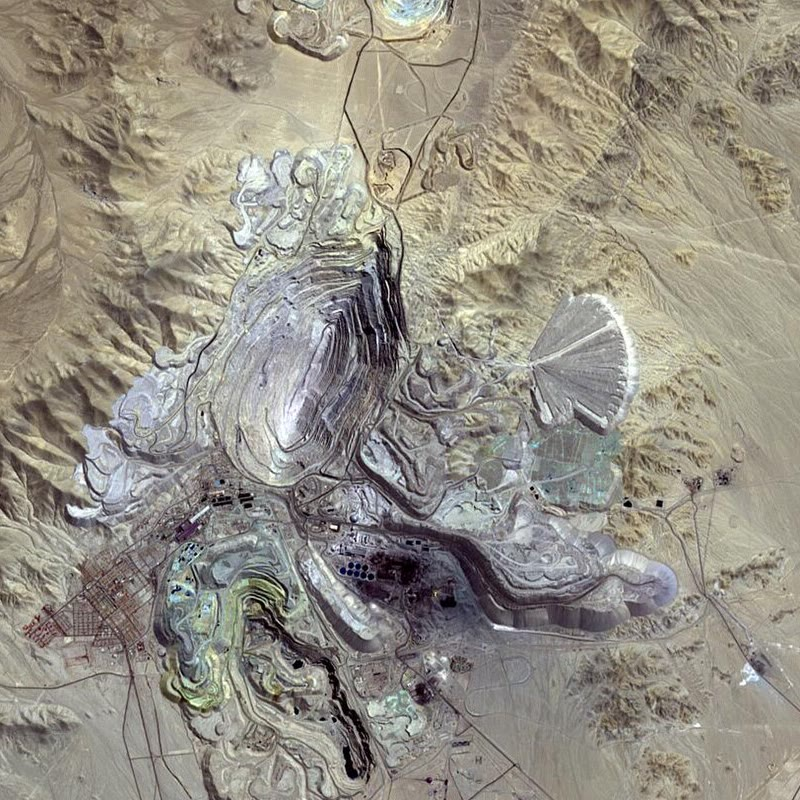
\includegraphics[width=\linewidth]{images/book1/g9-chuquicamata.jpg}
\end{minipage}\hfill
\begin{minipage}[c]{0.5\linewidth}\raggedright
{\small منجم النحاس في تشوكيكاماتا، في \omterm{def:g5:weather-and-climate:desert}{صحراء} أتاكاما في تشيلي، كما رآه
جهاز ASTER على قمر صناعي لوكالة ناسا في عام 2007 (يبلغ عرض الصورة نحو
\qty{12}{km}). والحفرة البيضوية في الوسط، المستغلة منذ أكثر من قرن،
طولها \qty{4.3}{km} وعرضها \qty{2.7}{km} وعمقها \qty{1.1}{km}.
ناسا وMETI وAIST ومنظومات اليابان الفضائية، وفريق ASTER العلمي
الأمريكي الياباني (ملك عام، عبر
ويكيميديا كومنز).}
\end{minipage}
% ledger: commons:chuquicamata, earle:chuquicamata
\label{fig:g9:earth-resources:chuquicamata}
\end{omfigure}

\paragraph{في حصباء الأنهار.} الذهب لا يصدأ ولا يكاد يتجوى. وحين تبري
\omterm{def:g5:water-shapes-the-land:erosion}{التعرية} عرقًا من الذهب، يتحرر الذهب غبارًا ورقائق وحبيبات وأحيانًا
كتلًا، وتحمله \omterm{def:g1:landscapes-around-us:water}{الأنهار} في اتجاه المصب. والذهب كثيف جدًا: نحو
\qty{19}{g/cm^3} للذهب الخالص، مقابل نحو \qty{2.5}{g/cm^3} \omterm{def:g3:stones-pebbles-sand:rock}{للصخر}
العادي. وفي \omterm{def:g5:water-shapes-the-land:flood}{الفيضانات}، حين يتحرك قاع \omterm{def:g3:stones-pebbles-sand:sand}{الرمل} \omterm{def:g3:stones-pebbles-sand:pebble}{والحصباء} كله، تشق حبيبات
الذهب الثقيلة طريقها إلى الأسفل وتتجمع على \omterm{def:g3:stones-pebbles-sand:rock}{الصخر الأساسي}. ويسمي
الجيولوجيون هذه المكامن \emph{الرواسب اللُّحَقية}\index{رواسب لحقية}.
% ledger: usgs:gold-placer

\section{الفحم والنفط والغاز}

الفحم والنفط والغاز الطبيعي بقايا كائنات حية، دُفنت قبل أن تتعفن.
فكل المادة العضوية لنبات أو حيوان ميت تقريبًا تعود ثاني أكسيد الكربون
في غضون أسابيع إلى عقود. ولا يمكن أن يُدفن ويُحفظ ملايين السنين إلا
الجزء المعزول عن أكسجين الهواء، في قاع مستنقع راكد أو \omterm{def:g2:water-on-earth:ocean}{بحر}
عميق.
% ledger: earle:coal, earle:oil-gas

\begin{omfigure}
\begin{minipage}[c]{0.46\linewidth}\centering
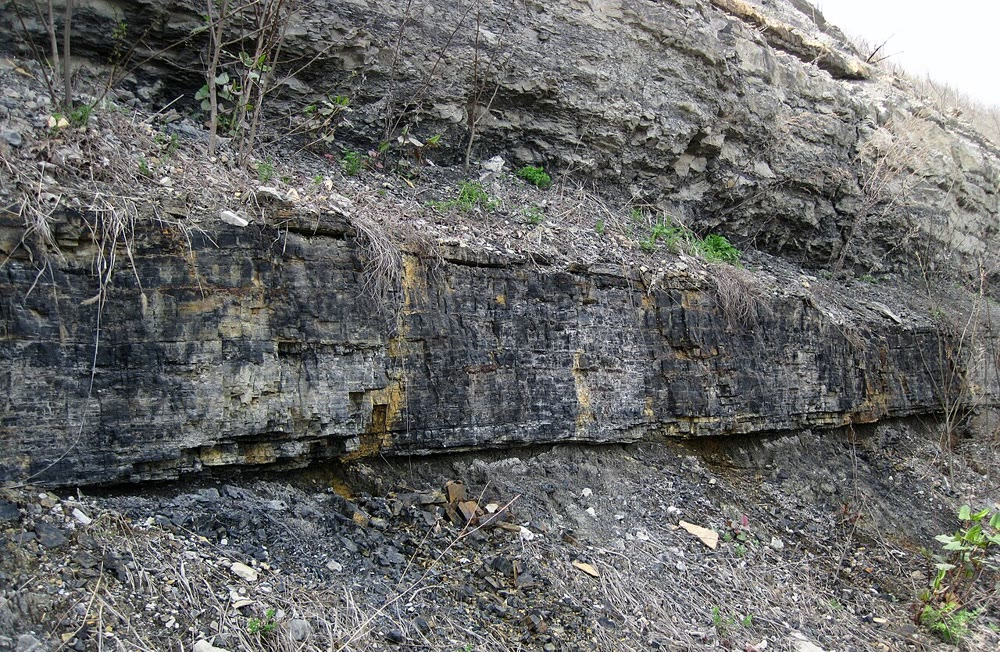
\includegraphics[width=\linewidth]{images/book1/g9-coal-seam.jpg}
\end{minipage}\hfill
\begin{minipage}[c]{0.5\linewidth}\raggedright
{\small طبقة من الفحم، هي الطبقة الداكنة التي تعبر الوسط، بين \omterm{def:g6:rocks-and-minerals:rock-families}{صخور
رسوبية}، بجانب طريق في أوهايو، الولايات المتحدة. والطبقة أفقية، كما كان
المستنقع. الصورة: جيمس سانت~جون (CC BY 2.0، عبر ويكيميديا
كومنز).}
\end{minipage}
% ledger: commons:meigs-coal
\label{fig:g9:earth-resources:coal-seam}
\end{omfigure}


\paragraph{الفحم.} يبدأ الفحم في المستنقعات المجاورة \omterm{def:g1:landscapes-around-us:water}{للأنهار} والدلتاوات،
في المناخات الحارة الرطبة، حيث تنمو النباتات بسرعة. فتسقط الجذوع
والأوراق الميتة في ماء راكد قليل الأكسجين، ولا تتعفن. ويجب أن يدوم
المستنقع قرونًا إلى آلاف السنين ليبني طبقة سميكة. وذات يوم يغيّر \omterm{def:g1:landscapes-around-us:water}{نهر}
مجراه أو يفيض، فيغطي المستنقع \omterm{def:g3:stones-pebbles-sand:sand}{بالرمل} \omterm{def:g3:stones-pebbles-sand:sand}{والوحل}. ومع تراكم مزيد من
\omterm{def:g7:sediments-and-fossils:sediment}{الرواسب}، تنضغط طبقة النباتات وتسخن، وتتحول إلى فحم: أولًا فحم بني طري
فيه نحو الثلث من الكربون، على عمق بضع مئات من الأمتار؛ ثم فحم أسود
صلب، فيه ما يصل إلى 86~\% من الكربون، على عمق بضعة كيلومترات. والفحم
المستخرج اليوم في الولايات المتحدة، مثلًا، عمره في الغالب بين 100
و300~مليون سنة.
% ledger: earle:coal, eia:coal

\begin{omfigure}
\begin{tikzpicture}[x=1cm, y=0.8cm, font=\footnotesize]
  \foreach \i/\t in {0/{\foreignlanguage{arabic}{\textdir TRT(أ) غابة مستنقعية}\\ تتراكم النباتات الميتة\\ تحت ماء راكد},
                     1/{\foreignlanguage{arabic}{\textdir TRT(ب) تُدفن تحت رمل}\\ النهر ووحله\\ فتنضغط الطبقة},
                     2/{\foreignlanguage{arabic}{\textdir TRT(ج) أعمق وأدفأ}\\ على مئات الأمتار\\ فحم بني طري},
                     3/{\foreignlanguage{arabic}{\textdir TRT(د) أعمق أيضًا}\\ على كيلومترات\\ فحم أسود صلب}} {
    \begin{scope}[xshift=\i*3.35cm]
      \draw[black!40] (0,0) rectangle (2.9,4.2);
      \node[align=center, anchor=north, font=\scriptsize] at (1.45,-0.1) {\t};
    \end{scope}
  }
  % (a) swamp: water, trees, plant layer
  \fill[omSea] (0,2.6) rectangle (2.9,3.1);
  \fill[brown!60!black!70] (0,2.0) rectangle (2.9,2.6);
  \fill[omLithShale] (0,0) rectangle (2.9,2.0);
  \foreach \x in {0.5,1.4,2.3} {
    \draw[brown!50!black, line width=1.2pt] (\x,2.6) -- (\x,3.7);
    \fill[green!45!black] (\x,3.85) circle (0.3);
  }
  % (b) buried
  \begin{scope}[xshift=3.35cm]
    \fill[lith sandstone] (0,2.6) rectangle (2.9,4.0);
    \fill[brown!55!black!80] (0,2.2) rectangle (2.9,2.6);
    \fill[omLithShale] (0,0) rectangle (2.9,2.2);
    \draw[->, thick] (1.45,4.15) -- (1.45,3.45);
  \end{scope}
  % (c) lignite
  \begin{scope}[xshift=6.7cm]
    \fill[lith sandstone] (0,1.9) rectangle (2.9,4.2);
    \fill[brown!45!black] (0,1.65) rectangle (2.9,1.9);
    \fill[omLithShale] (0,0) rectangle (2.9,1.65);
  \end{scope}
  % (d) coal
  \begin{scope}[xshift=10.05cm]
    \fill[lith sandstone] (0,1.25) rectangle (2.9,4.2);
    \fill[black!85] (0,1.1) rectangle (2.9,1.25);
    \fill[omLithShale] (0,0) rectangle (2.9,1.1);
  \end{scope}
\end{tikzpicture}

{\small من المستنقع إلى طبقة الفحم (رسم تخطيطي، ليس بمقياس رسم). كلما
غاصت طبقة النباتات أعمق، انضغطت وسخنت: فيغادرها الماء والغازات، وترقّ،
وترتفع حصة الكربون فيها.}
% ledger: earle:coal, eia:coal
\label{fig:g9:earth-resources:coal}
\end{omfigure}


\paragraph{النفط والغاز.} يأتي النفط ومعظم الغاز الطبيعي من النباتات
والحيوانات الدقيقة التي تعيش في \omterm{def:g2:water-on-earth:ocean}{البحر}، مثل الدياتومات. فتهبط بقاياها
مع \omterm{def:g3:stones-pebbles-sand:sand}{الوحل} إلى قاع \omterm{def:g2:water-on-earth:ocean}{البحر}، ويُدفن بعضها قبل أن يتحلل. وبعد ملايين السنين
وكيلومترات من \omterm{def:g7:sediments-and-fossils:sediment}{الرواسب}، تغيّرها الحرارة والضغط: فتحت نحو \qty{2}{km}،
بين نحو 60 و\qty{120}{\degreeCelsius}، تصير نفطًا؛ وفي حرارة أعلى،
غازًا. والنفط والغاز أخف من الماء. فيزحفان ببطء نحو الأعلى عبر \omterm{def:g6:water-underground:porosity}{مسام}
\omterm{def:g3:stones-pebbles-sand:rock}{الصخور} \omterm{def:g6:water-underground:permeability}{النفوذة}، ويبلغ كثير منهما السطح ويضيع. أما ما نجده فقد أوقفته
في طريقه طبقة من \omterm{def:g3:stones-pebbles-sand:rock}{صخر} \omterm{def:g6:water-underground:permeability}{كتيم}، كثيرًا ما تكون في قمة طية مقوّسة إلى أعلى،
حيث يتجمعان: الغاز في الأعلى، والنفط تحته، والماء
أسفلهما.
% ledger: eia:oil, eia:gas, earle:oil-gas

\begin{omfigure}
\begin{tikzpicture}[x=1cm, y=1cm, font=\footnotesize, >={Stealth[length=2mm]}]
  \def\fold#1{(0,#1) .. controls (3,#1+1.0) and (4.0,#1+1.6) .. (6,#1+1.6) .. controls (8.0,#1+1.6) and (9,#1+1.0) .. (12,#1)}
  % layers from the bottom up
  \fill[omLithShale!60!black!40] (0,0) -- \fold{0.9} -- (12,0) -- cycle;
  \fill[lith sandstone] \fold{0.9} -- (12,2.1) -- (12,2.1) .. controls (9,3.1) and (8.0,3.7) .. (6,3.7) .. controls (4.0,3.7) and (3,3.1) .. (0,2.1) -- cycle;
  \fill[lith shale] (0,2.1) .. controls (3,3.1) and (4.0,3.7) .. (6,3.7) .. controls (8.0,3.7) and (9,3.1) .. (12,2.1) -- (12,3.6) .. controls (9,4.6) and (8.0,5.2) .. (6,5.2) .. controls (4.0,5.2) and (3,4.6) .. (0,3.6) -- cycle;
  \fill[lith sandstone] (0,3.6) .. controls (3,4.6) and (4.0,5.2) .. (6,5.2) .. controls (8.0,5.2) and (9,4.6) .. (12,3.6) -- (12,5.6) -- (0,5.6) -- cycle;
  % gas and oil under the crest of the impermeable layer
  \fill[omWxSun!60] (4.55,3.55) .. controls (5.2,3.69) and (6.8,3.69) .. (7.45,3.55) -- (7.1,3.35) -- (4.9,3.35) -- cycle;
  \fill[black!75] (4.9,3.35) -- (7.1,3.35) -- (8.05,3.05) .. controls (7.0,3.15) and (5.0,3.15) .. (3.95,3.05) -- cycle;
  % arrows: oil creeping up through the permeable layer
  \draw[->, black, thick] (1.4,2.05) -- (2.4,2.55);
  \draw[->, black, thick] (10.6,2.05) -- (9.6,2.55);
  \draw[->, black!70] (3.0,2.65) -- (3.8,2.95);
  \draw[->, black!70] (9.0,2.65) -- (8.2,2.95);
  % labels
  \node[anchor=west, fill=white, fill opacity=0.85, text opacity=1, inner sep=1.5pt] at (0.1,0.45) {الوحل الداكن لقاع البحر القديم: هنا يتكوّن النفط والغاز};
  \node[anchor=east, fill=white, fill opacity=0.85, text opacity=1, inner sep=1.5pt] at (11.9,1.9) {حجر رملي نفوذ};
  \node[anchor=east, fill=white, fill opacity=0.85, text opacity=1, inner sep=1.5pt] at (11.9,3.25) {سجّيل كتيم};
  \node[anchor=south, fill=white, fill opacity=0.85, text opacity=1, inner sep=1.5pt] at (6,5.25) {صخور السطح};
  \node[font=\scriptsize] at (6,3.48) {غاز};
  \node[font=\scriptsize, text=white] at (6,3.22) {نفط};
\end{tikzpicture}

{\small نفط وغاز أوقفتهما طبقة \omterm{def:g6:water-underground:permeability}{كتيمة} في قمة طية مقوّسة إلى أعلى (رسم
تخطيطي، ليس بمقياس رسم؛ والماء الذي يملأ بقية الحجر الرملي غير مرسوم).
وتحت الطية، يزحفان صعودًا عبر الحجر الرملي \omterm{def:g6:water-underground:permeability}{النفوذ} (الأسهم) ويتجمعان
تحت القمة: الغاز في الأعلى، والنفط
تحته.}
% ledger: earle:oil-gas
\label{fig:g9:earth-resources:oil}
\end{omfigure}

\section{الماء من باطن الأرض}

\omterm{def:g6:water-underground:groundwater}{المياه الجوفية} أيضًا مورد من الأرض، وهو المورد الذي نستعمله كل يوم.
وخلافًا للفلز أو الفحم، فهي تتجدد: \omterm{def:g4:clouds-rain-snow:precipitation}{فالمطر} يعيد ملء الخزانات الجوفية.
لكنها تتجدد ببطء، ولا تتجدد إلا بالسرعة التي يتسرب بها \omterm{def:g4:clouds-rain-snow:precipitation}{المطر}. \omterm{def:g6:water-underground:aquifer}{والخزان
الجوفي} الذي يُضخ أسرع مما يُعاد ملؤه ينخفض منسوب مياهه الجوفية، وتجف
\omterm{def:g6:water-underground:spring}{الآبار} (\cref{ch:g6:water-underground}). \omterm{def:g6:water-underground:groundwater}{فالمياه الجوفية} مورد متجدد ما
دامت لا تُسحب أسرع مما تتجدد.
% ledger: wss:aquifer

\section{الرمل والحصباء}

المادة الصلبة التي يستخرجها الناس من الأرض بأكبر الكميات ليست الفحم
ولا خام فلز: إنها \omterm{def:g3:stones-pebbles-sand:sand}{الرمل} \omterm{def:g3:stones-pebbles-sand:pebble}{والحصباء}.
% ledger: tos:sand

\begin{definition}[الحصويات]\label{def:g9:earth-resources:aggregate}
\emph{الحصويات}\index{حصويات} هي \omterm{def:g3:stones-pebbles-sand:sand}{الرمل} \omterm{def:g3:stones-pebbles-sand:pebble}{والحصباء} والحجر المكسّر المستعملة
في البناء: في الخرسانة، وتحت الطرق والسكك الحديدية، ولردم
الأرض.
\end{definition}
% ledger: usgs:aggregate, tos:sand

يذهب معظم \omterm{def:g3:stones-pebbles-sand:sand}{الرمل} إلى الخرسانة، وهي مزيج من \omterm{def:g3:stones-pebbles-sand:sand}{الرمل} \omterm{def:g3:stones-pebbles-sand:pebble}{والحصباء} والماء
والإسمنت. وفي عام 2019 احتاج العالم إلى نحو 50~مليار طن من \omterm{def:g3:stones-pebbles-sand:sand}{الرمل}
\omterm{def:g3:stones-pebbles-sand:pebble}{والحصباء} في السنة، أي $5 \times 10^{10}$ طن، أو نحو \qty{18}{kg} لكل
إنسان على الأرض، كل يوم. ويُستخرج \omterm{def:g3:stones-pebbles-sand:sand}{الرمل} \omterm{def:g3:stones-pebbles-sand:pebble}{والحصباء} من حفر على اليابسة،
ومن قيعان \omterm{def:g1:landscapes-around-us:water}{الأنهار}، ومن قاع \omterm{def:g2:water-on-earth:ocean}{البحر} أكثر فأكثر. وحين يؤخذان من \omterm{def:g1:landscapes-around-us:water}{نهر}، يقل
\omterm{def:g3:stones-pebbles-sand:sand}{الرمل} الذي يبلغ \omterm{def:g1:landscapes-around-us:water}{الساحل}، فتتآكل الشواطئ الواقعة في اتجاه المصب.
% ledger: tos:sand

\begin{omfigure}
\begin{minipage}[c]{0.46\linewidth}\centering
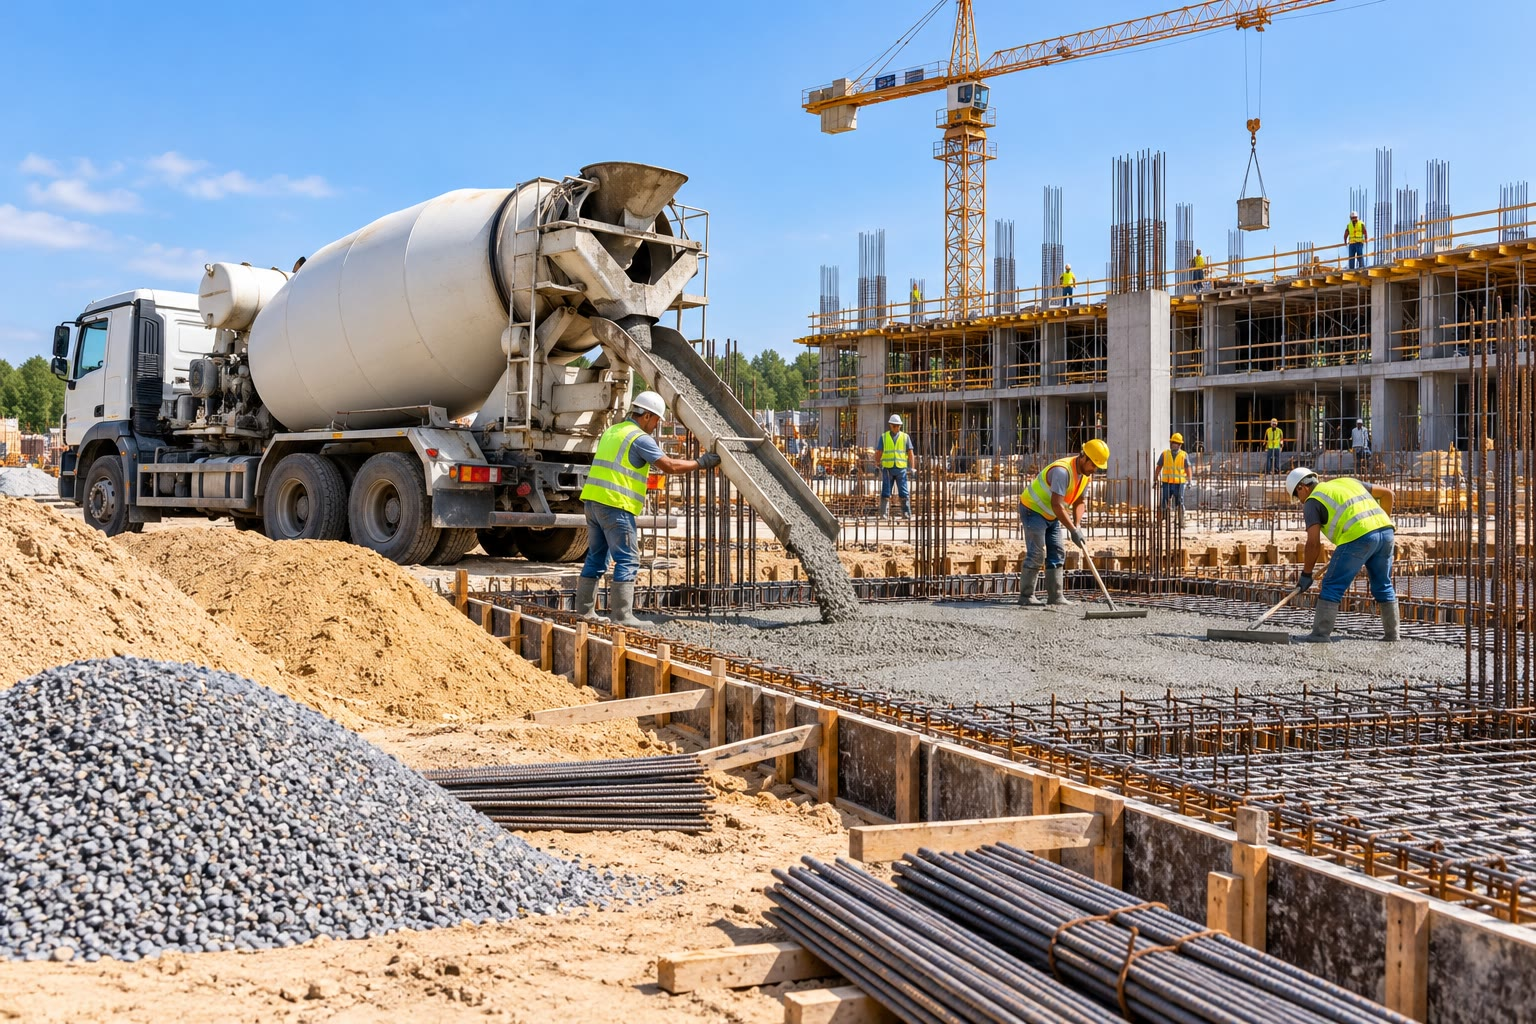
\includegraphics[width=\linewidth]{images/book1/ai/g9-building-site.jpg}
\end{minipage}\hfill
\begin{minipage}[c]{0.5\linewidth}\raggedright
{\small \omterm{def:g9:earth-resources:aggregate}{الحصويات} في العمل: أكوام من \omterm{def:g3:stones-pebbles-sand:sand}{الرمل} \omterm{def:g3:stones-pebbles-sand:pebble}{والحصباء} بجانب شاحنة خلط
خرسانة تصب أرضية مبنى جديد (رسم توضيحي مولَّد بالذكاء الاصطناعي لمشهد
عام).}
\end{minipage}
\label{fig:g9:earth-resources:building-site}
\end{omfigure}

\section{متجدد أم محدود؟}

المورد الذي تجدده الطبيعة في مدى عمر إنسان، مثل ماء \omterm{def:g6:water-underground:aquifer}{خزان جوفي} لا
يُفرط في ضخه، يمكن أن يُستعمل إلى الأبد. أما \omterm{def:g9:earth-resources:ore-deposit}{مكمن الخام}، أو طبقة الفحم
أو حقل النفط، فقد استغرق تكوينه ملايين السنين. ونحن نستهلكه في بضعة
عقود: فعلى سلّمنا الزمني، لا يتجدد أبدًا.
% ledger: eia:coal, earle:coal

\begin{omfigure}
\begin{tikzpicture}
\begin{axis}[xmode=log, width=12.5cm, height=4.6cm, xmin=10, xmax=1e9, ymin=0.4, ymax=4.6,
  ytick=\empty, xlabel={\foreignlanguage{arabic}{السنوات، بسلّم لوغاريتمي}}, label style={font=\small},
  xtick={10,100,1000,1e4,1e5,1e6,1e7,1e8,1e9},
  xticklabels={$10$,$10^2$,$10^3$,$10^4$,$10^5$,$10^6$,$10^7$,$10^8$,$10^9$},
  tick label style={font=\footnotesize}, xmajorgrids, grid style={black!12}, clip=false]
\addplot[only marks, mark=|, mark size=4pt, line width=4pt, omWarm,
  error bars/.cd, x dir=plus, x explicit, error bar style={line width=4pt, omWarm}, error mark=none]
  table[x=lo_yr, y=y, x error expr=\thisrow{hi_yr}-\thisrow{lo_yr}] {figdata/out/grade-9-concentration-times.dat};
\node[anchor=west, font=\footnotesize, fill=white, inner sep=1pt] at (axis cs:1500,4) {مستنقع يبني طبقة سميكة من النباتات};
\node[anchor=east, font=\footnotesize, fill=white, inner sep=1pt] at (axis cs:6e7,3) {عمر الفحم المستخرج في الولايات المتحدة};
\node[anchor=west, font=\footnotesize, fill=white, inner sep=1pt] at (axis cs:150,2) {\foreignlanguage{arabic}{استغلال تشوكيكاماتا حتى الآن: أكثر من قرن}};
\node[anchor=west, font=\footnotesize, fill=white, inner sep=1pt] at (axis cs:65,1) {\foreignlanguage{arabic}{احتياطيات النحاس العالمية بوتيرة تعدين \babelsublr{2024}}};
\end{axis}
\end{tikzpicture}

{\small أزمنة التكوين وأزمنة الاستهلاك، على سلّم كل درجة فيه عشرة أضعاف
التي قبلها. فالفحم أقدم بنحو مليون مرة من الزمن الذي يستغرقه منجم
ليُفرغ مكمنًا.}
% ledger: earle:coal, eia:coal, earle:chuquicamata, usgs:mcs-copper (figdata/grade-9/concentration.py, part times)
\label{fig:g9:earth-resources:times}
\end{omfigure}

كم سيدوم مورد ما؟ لا يحسب الجيولوجيون إلا ما هو معروف ويمكن
استخراجه.

\begin{definition}[الاحتياطي]\label{def:g9:earth-resources:reserve}
\emph{الاحتياطي}\index{احتياطي} من مورد معدني هو الجزء من المكامن
المعروفة الذي يمكن استخراجه بربح، بتقنيات اليوم
وأسعاره.
\end{definition}
% ledger: usgs:mcs-reserves

\omterm{def:g9:earth-resources:reserve}{الاحتياطي} ليس كل ما في الأرض. فهو يكبر حين تُكتشف مكامن جديدة، أو
تتحسن التقنيات، أو ترتفع الأسعار، ويصغر كلما استُغلت المكامن. ففي عام
1970 قُدّرت \omterm{def:g9:earth-resources:reserve}{احتياطيات} النحاس في العالم بما مقداره 280~مليون طن. ومنذ
ذلك الحين، استُخرج نحو 700~مليون طن من النحاس، أي ما يعادل ذلك
\omterm{def:g9:earth-resources:reserve}{الاحتياطي} مرتين ونصفًا، ومع ذلك قُدّرت \omterm{def:g9:earth-resources:reserve}{احتياطيات} عام 2024 بما مقداره
980~مليون طن.
% ledger: usgs:mcs-reserves

\begin{dated}{2025}
في عام 2024 أنتجت مناجم العالم نحو 23~مليون طن من النحاس.
وبهذه الوتيرة، تكفي \omterm{def:g9:earth-resources:reserve}{الاحتياطيات} البالغة 980~مليون طن $980 \div 23
\approx 43$ سنة. وليس هذا العدد تاريخًا ينفد فيه النحاس: بل هو مقياس
للنحاس المعروف والذي يستحق الاستخراج اليوم.
\end{dated}
% ledger: usgs:mcs-copper (figdata/grade-9/concentration.py: 42.6 years)

الفلز، خلافًا للفحم أو النفط، لا يُتلف حين يُستعمل: فإعادة تدوير
المواد، التي تعرّفتها في كتب الكيمياء، تعيده إلينا. فنحاس كابل قديم، أو
محرك مُخرَّد، أو قصاصات مصنع، يمكن صهره وتكريره من جديد. وفي الولايات
المتحدة في عام 2024، شكّل النحاس المستعاد من الخردة نحو \qty{35}{\%}
من كل النحاس
المستعمل.
% ledger: usgs:mcs-copper-scrap

\begin{omfigure}
\begin{tikzpicture}[font=\footnotesize, node distance=1.2cm,
  box/.style={draw=black!60, fill=black!4, rounded corners=2pt, align=center, minimum height=0.9cm, inner sep=3pt},
  flow/.style={-{Stealth[length=2.2mm]}, line width=0.9pt, black!70}]
  \node[box, fill=omWarm!12] (ore) at (0,0) {مكمن خام\\\foreignlanguage{arabic}{صخر فيه \qty{0.5}{\%}}\\من النحاس};
  \node[box] (metal) at (4.2,0) {النحاس الفلزي};
  \node[box] (things) at (8.2,0) {كابلات وأنابيب\\ومحركات};
  \node[box, fill=blue!8] (scrap) at (6.2,-2.1) {خردة};
  \node[box, fill=black!12] (waste) at (0,-2.1) {صخر مسحوق\\متبقٍّ};
  \draw[flow] (ore) -- node[above] {حفر وسحق} node[below] {ثم تركيز} (metal);
  \draw[flow] (metal) -- node[above] {تصنيع} (things);
  \draw[flow] (things) |- node[pos=0.25, right] {يُرمى} (scrap);
  \draw[flow] (scrap) -| node[pos=0.75, left] {صهر وتكرير} (metal);
  \draw[flow] (ore) -- (waste);
\end{tikzpicture}

{\small طريقان إلى النحاس الفلزي: من خام، عبر أطنان من \omterm{def:g3:stones-pebbles-sand:rock}{الصخر} المحفور
والمسحوق، أو من الخردة، التي تُصهر وتُكرَّر من جديد.}
\end{omfigure}

\begin{example}[الصخر الذي توفّره إعادة التدوير]\label{ex:g9:earth-resources:recycling}
الخام الذي فيه \qty{0.5}{\%} من النحاس يحوي \qty{5}{kg} من النحاس في كل
طن من \omterm{def:g3:stones-pebbles-sand:rock}{الصخر}. ولصنع طن واحد من النحاس، يجب حفر نحو $1000 \div 5 = 200$
طن من الخام وسحقها ومعالجتها، وينتهي معظمها تقريبًا \omterm{def:g3:stones-pebbles-sand:rock}{صخرًا} مُهملًا. وكل
طن من النحاس يُصنع من الخردة يترك في الأرض 200 طن من \omterm{def:g3:stones-pebbles-sand:rock}{الصخر} --- ويدوم
المكمن مدة أطول.
% ledger: perkins:ore-grades (computed)
\end{example}


\section{تمارين}

\begin{exercise}[$\star$]\label{exo:g9:earth-resources:1}
أكمل بالكلمة المناسبة (\omterm{def:g9:earth-resources:ore-deposit}{مكمن خام}، \omterm{def:g9:earth-resources:ore-deposit}{معامل تركيز}، \omterm{def:g9:earth-resources:aggregate}{حصويات}، \omterm{def:g9:earth-resources:reserve}{احتياطي}).
(أ) \omterm{def:g3:stones-pebbles-sand:sand}{الرمل} المستعمل في الخرسانة من \ldots\ (ب) الجزء من النحاس المعروف
الذي يمكن استخراجه بربح اليوم هو \ldots\ النحاس. (ج) \omterm{def:g3:stones-pebbles-sand:rock}{الصخر} الذي يكون
فيه فلز غنيًا بما يكفي لتعدينه هو \ldots\ (د) عدد المرات التي تركّز
بها فلز هو \ldots
\end{exercise}

\begin{exercise}[$\star$]\label{exo:g9:earth-resources:2}
% ledger: earle:magmatic, usgs:gold-lode, usgs:gold-placer
أي طريقة لتركيز الفلز تصفها كل جملة: في \omterm{def:g7:volcanoes:magma}{الصهارة}، أم في الشقوق من الماء
الحار، أم في \omterm{def:g3:stones-pebbles-sand:pebble}{حصباء} \omterm{def:g1:landscapes-around-us:water}{الأنهار}؟ (أ) كتل من الذهب ترقد على \omterm{def:g3:stones-pebbles-sand:rock}{الصخر الأساسي}
تحت \omterm{def:g3:stones-pebbles-sand:pebble}{حصباء} جدول. (ب) ماء حار يملأ شقًا بالكوارتز والذهب. (ج) طبقة من
\omterm{def:g6:rocks-and-minerals:mineral}{معادن} النيكل الثقيلة ترقد في قاع جسم قديم من \omterm{def:g7:volcanoes:magma}{الصهارة}. (د) يتحرر الذهب
من عرق معدني \omterm{def:g5:water-shapes-the-land:erosion}{بالتعرية}.
\end{exercise}

\begin{exercise}[$\star$]\label{exo:g9:earth-resources:3}
% ledger: earle:coal, eia:coal
رتّب هذه المراحل: (أ) تُدفن طبقة النباتات تحت \omterm{def:g3:stones-pebbles-sand:sand}{رمل} \omterm{def:g1:landscapes-around-us:water}{النهر}؛ (ب) تنمو
الأشجار في مستنقع؛ (ج) يتكوّن فحم أسود صلب على عمق كيلومترات؛ (د) تتراكم
النباتات الميتة تحت ماء راكد؛ (ه) يتكوّن فحم بني طري.
\end{exercise}

\begin{exercise}[$\star$]\label{exo:g9:earth-resources:4}
على سلّم حياة الإنسان، هل كل مورد من هذه الموارد متجدد أم لا؟ اشرح في
جملة واحدة. (أ) الفحم. (ب) ماء \omterm{def:g6:water-underground:aquifer}{خزان جوفي} يُضخ منه أقل مما يعيد \omterm{def:g4:clouds-rain-snow:precipitation}{المطر}
ملأه. (ج) خام النحاس. (د) \omterm{def:g6:water-underground:aquifer}{الخزان الجوفي} نفسه يُضخ بضعف سرعة إعادة
ملئه.
\end{exercise}

\begin{exercise}[$\star\star$]\label{exo:g9:earth-resources:5}
% ledger: perkins:ore-grades
احسب \omterm{def:g9:earth-resources:ore-deposit}{معامل التركيز}، ثم اكتبه قوةً للعدد عشرة، مقرَّبًا: (أ) الزنك،
\qty{0.007}{\%} في \omterm{def:g6:inside-the-earth:layers}{القشرة}، وخامه ابتداءً من \qty{4}{\%}؛ (ب) القصدير،
\qty{0.0002}{\%} في \omterm{def:g6:inside-the-earth:layers}{القشرة}، وخامه ابتداءً من \qty{0.5}{\%}؛ (ج) الحديد،
\qty{5.6}{\%} في \omterm{def:g6:inside-the-earth:layers}{القشرة}، وخامه ابتداءً من \qty{20}{\%}. (د) لماذا يحتاج
الحديد إلى تركيز قليل جدًا؟
\end{exercise}

\begin{exercise}[$\star\star$]\label{exo:g9:earth-resources:6}
% ledger: usgs:gold-placer
كثافة الذهب الخالص نحو \qty{19.3}{g/cm^3}؛ \omterm{def:g3:stones-pebbles-sand:rock}{والصخر} العادي نحو
\qty{2.5}{g/cm^3}. (أ) كم مرة يكون الذهب أكثف؟ (ب) ما كتلة حبيبة ذهب
حجمها \qty{0.01}{cm^3}، وما كتلة حبيبة \omterm{def:g3:stones-pebbles-sand:rock}{صخر} لها الحجم نفسه؟ (ج) اشرح
لماذا ينتهي الذهب، في \omterm{def:g5:water-shapes-the-land:flood}{الفيضان}، في أسفل \omterm{def:g3:stones-pebbles-sand:pebble}{الحصباء}، على \omterm{def:g3:stones-pebbles-sand:rock}{الصخر
الأساسي}.
\end{exercise}

\begin{exercise}[$\star\star$]\label{exo:g9:earth-resources:7}
% ledger: perkins:ore-grades, earle:ore-grades (figdata/grade-9/concentration.py)
استعمل الرسم البياني لمعاملات التركيز. (أ) أي الفلزات تحتاج إلى معامل
أكبر من $10^3$؟ (ب) بين أي قوتين للعدد عشرة يقع النحاس؟ (ج) كم
مرة يجب أن يتركز الكروم أكثر من الألومنيوم؟ (د) أي الفلزات السبعة
تتوقع أن تجده مستخرجًا في أقل عدد من الأماكن؟
علّل.
\end{exercise}

\begin{exercise}[$\star\star$]\label{exo:g9:earth-resources:8}
% ledger: tos:sand
يحتاج العالم إلى نحو \qty{18}{kg} من \omterm{def:g3:stones-pebbles-sand:sand}{الرمل} \omterm{def:g3:stones-pebbles-sand:pebble}{والحصباء} للشخص الواحد في
اليوم. (أ) كم يبلغ ذلك للشخص في سنة واحدة، بالأطنان؟ (ب) اكتب 50 مليار
طن بالترميز العلمي. (ج) تحمل شاحنة \qty{25}{t}. كم يومًا يلزم كي
يملأها نصيب شخص واحد؟ (د) لماذا يمكن أن يؤدي أخذ \omterm{def:g3:stones-pebbles-sand:sand}{الرمل} من \omterm{def:g1:landscapes-around-us:water}{نهر} إلى
تقلص شاطئ في اتجاه المصب؟
\end{exercise}

\begin{exercise}[$\star\star$]\label{exo:g9:earth-resources:9}
% ledger: earle:oil-gas, eia:oil
(أ) من أي كائنات حية يأتي معظم النفط والغاز؟ (ب) تحت نحو \qty{2}{km}،
في أي درجات حرارة يتكوّن النفط؟ (ج) لماذا يتحرك النفط والغاز نحو الأعلى
عبر \omterm{def:g3:stones-pebbles-sand:rock}{الصخور}؟ (د) أي نوع من \omterm{def:g3:stones-pebbles-sand:rock}{الصخر} يوقفهما، وأين
يتجمعان؟
\end{exercise}

\begin{exercise}[$\star\star$]\label{exo:g9:earth-resources:10}
% ledger: earle:chuquicamata
أنتج منجم تشوكيكاماتا أكثر من 29~مليون طن من النحاس في أكثر من 100
سنة. (أ) اكتب 29~مليون طن بالترميز العلمي. (ب) ما متوسط الإنتاج في
السنة تقريبًا؟ (ج) لو كان الخام يحوي \qty{1}{\%} من النحاس، فكم طنًا من
الخام حُفر للحصول على 29~مليون طن من النحاس؟ استعمل الترميز العلمي.
(د) لماذا يجب أن يكون منجم خامٍ بهذا الفقر كبيرًا إلى هذا
الحد؟
\end{exercise}

\begin{exercise}[$\star\star\star$]\label{exo:g9:earth-resources:11}
% ledger: usgs:mcs-reserves, usgs:mcs-copper
في عام 1970، قُدّرت \omterm{def:g9:earth-resources:reserve}{احتياطيات} النحاس في العالم بما مقداره 280~مليون
طن. ومن 1970 إلى 2024، استُخرج نحو 697~مليون طن، وكانت \omterm{def:g9:earth-resources:reserve}{احتياطيات} عام
2024 تبلغ 980~مليون طن، مع استخراج 23~مليون طن في عام 2024. (أ) لو كان
\omterm{def:g9:earth-resources:reserve}{احتياطي} 1970 هو كل النحاس الموجود، فمتى كان سينفد؟ قارن بما استُخرج.
(ب) كم مرة يكبر \omterm{def:g9:earth-resources:reserve}{احتياطي} 2024 \omterm{def:g9:earth-resources:reserve}{احتياطي} 1970؟ (ج) احسب كم سنة يكفي
\omterm{def:g9:earth-resources:reserve}{احتياطي} 2024 بوتيرة 2024. (د) اذكر سببين يجعلان \omterm{def:g9:earth-resources:reserve}{الاحتياطي} يكبر حتى وهو
يُستغل.
\end{exercise}

\begin{exercise}[$\star\star\star$]\label{exo:g9:earth-resources:12}
% ledger: earle:coal, eia:coal
عمر طبقة فحم $3 \times 10^8$ سنة. ودام مستنقعها $2 \times 10^3$
سنة، وتُستنفد الطبقة بالتعدين في 50 سنة. (أ) اكتب 50 سنة بالترميز
العلمي. (ب) كم مرة دام المستنقع أطول من مدة التعدين؟ (ج) كم مرة تكون
الطبقة أقدم من مدة التعدين؟ (د) استعمل هذه الأعداد لتشرح لماذا يُسمى
الفحم موردًا غير
متجدد.
\end{exercise}

\section{مسألة: خرسانة لمدينة جديدة}

\begin{problem}[{مسألة نهاية الأسبوع --- تُبنى مدينة جديدة برمل حفرة
محلية؛ والجواب الأخير هو عدد السنوات التي يكفيها احتياطي الرمل في
الحفرة}]
\label{pb:g9:earth-resources:1}
% ledger: usgs:aggregate (about 100 and 300 t per home), tos:sand (figdata/grade-9/concentration.py, part problem: exercise data)
ستُبنى مدينة جديدة من \num{2000} مسكن في عشر سنوات، قرب حفرة \omterm{def:g3:stones-pebbles-sand:sand}{رمل} قديمة
محفورة في \omterm{def:g3:stones-pebbles-sand:pebble}{حصباء} مصطبة نهرية. ومع حساب نصيبه من الشوارع والمدارس
والمتاجر، يحتاج كل مسكن إلى نحو \qty{300}{t} من \omterm{def:g9:earth-resources:aggregate}{الحصويات}،
\qty{40}{\%} منها \omterm{def:g3:stones-pebbles-sand:sand}{رمل}. وطبقة \omterm{def:g3:stones-pebbles-sand:sand}{الرمل} في الحفرة طولها \qty{1.2}{km}
وعرضها \qty{500}{m} وسمكها \qty{5}{m}؛ وكتلة المتر المكعب الواحد من
رملها \qty{1.6}{t}. وتبيع الحفرة أيضًا \num{136000} طن من \omterm{def:g3:stones-pebbles-sand:sand}{الرمل} في
السنة لبقية المنطقة.

\noindent\textbf{الجزء الأول --- كم من الرمل؟}\par\nopagebreak
\begin{enumerate}[beginpenalty=10000]
  \item يحتاج بيت أسرة وحده إلى نحو \qty{100}{t} من \omterm{def:g9:earth-resources:aggregate}{الحصويات}. اكتب
        هذه الكتلة بالكيلوغرامات، بالترميز العلمي.
  \item كم طنًا من \omterm{def:g9:earth-resources:aggregate}{الحصويات} ستحتاج المدينة كلها؟
  \item كم طنًا يساوي ذلك في السنة، على مدى السنوات العشر؟
  \item كم طنًا من \omterm{def:g3:stones-pebbles-sand:sand}{الرمل} تحتاج المدينة في السنة؟
\end{enumerate}

\noindent\textbf{الجزء الثاني --- الاحتياطي.}\par\nopagebreak
\begin{enumerate}[resume, beginpenalty=10000]
  \item احسب حجم طبقة \omterm{def:g3:stones-pebbles-sand:sand}{الرمل}، بالأمتار المكعبة، بالترميز
        العلمي.
  \item يقع ثلث الطبقة تحت قرية وطريق ولن يُحفر. ما الحجم
        الذي يمكن استخراجه؟
  \item ما كتلة هذا \omterm{def:g9:earth-resources:reserve}{الاحتياطي}، بالأطنان؟
  \item كم طنًا من \omterm{def:g3:stones-pebbles-sand:sand}{الرمل} ستبيع الحفرة كل سنة، للمدينة وللمنطقة
        معًا؟
\end{enumerate}

\noindent\textbf{الجزء الثالث --- متجدد أم لا؟}\par\nopagebreak
\begin{enumerate}[resume, beginpenalty=10000]
  \item كل سنة، يجلب \omterm{def:g1:landscapes-around-us:water}{النهر} نحو \num{2000} طن من \omterm{def:g3:stones-pebbles-sand:sand}{الرمل} الجديد إلى
        المنطقة. كم مرة تبيع الحفرة أكثر من ذلك؟
  \item على سلّم حياة المدينة، هل هذا \omterm{def:g3:stones-pebbles-sand:sand}{الرمل} مورد متجدد؟
        علّل.
  \item لو استبدلت المدينة بربع رملها خرسانة قديمة مسحوقة، فكم طنًا
        من \omterm{def:g3:stones-pebbles-sand:sand}{الرمل} ستوفر كل سنة؟
  \item من دون إعادة التدوير هذه، كم سنة يكفي \omterm{def:g9:earth-resources:reserve}{احتياطي} \omterm{def:g3:stones-pebbles-sand:sand}{الرمل} في
        الحفرة؟
\end{enumerate}
\end{problem}
